\documentclass[12pt]{article}
\usepackage{url, graphicx}
\usepackage{geometry}
\usepackage{amsmath}
\usepackage{fancyhdr}
\usepackage{nopageno}
\usepackage[usenames, dvipsnames]{color}

\pagestyle{fancy}

\title{\huge Lecture 6: Recursive Algorithms: Finding the Closest Pair of Points}
\author{}
\date{}
\pagestyle{fancy}
\fancyhf{}
\lhead{COMP 251 Winter 2018}
\rhead{Lecture 6}
\lfoot{$19^{th}$ Jan, 2018}
\rfoot{\copyright{}Yutong Yan}
\newcommand{\forceindent}{\leavevmode{\parindent=1em\indent}}
\begin{document}
\maketitle
\section{Finding the Closest Pair of Points in the Plane}
\renewcommand{\labelitemii}{$\circ$}
\renewcommand{\labelitemiii}{$\cdot$}
\renewcommand{\labelitemiii}{$\rightarrow$}
\renewcommand{\labelitemiv}{$\star$}
\begin{itemize}
\item Given n points $P = \{p_1, p_2, \cdot \cdot \cdot p_n\}$. find the \textbf{closest} pair of points.
\item We will investigate the case where the points are in the plane.
	\begin{itemize}
	\item The point set is 2-dimensional.
	\item Specifically, for each $1 \leq i \leq n$, let $P_i = (x_i. y_i)$.
	\end{itemize}
\item How quickly can we do?
\end{itemize}

\section{Exhaustive Search}
\renewcommand{\labelitemii}{$\circ$}
\renewcommand{\labelitemiii}{$\cdot$}
\renewcommand{\labelitemiii}{$\rightarrow$}
\renewcommand{\labelitemiv}{$\star$}
\begin{itemize}
\item The simplest algorithm to try is \textbf{exhaustive search}:
	\begin{itemize}
	\item Calculate the distance between \underline{every} pair of points.
	\item Output the pair with the \textit{shortest pairwise distance}. 
	\end{itemize}
\item What is the running time?
	\begin{itemize}
	\item There are n points so there are {\large $\binom{n}{2} = \frac{n \cdot (n - 1)}{2}$} pairs of points.
	\item Runtime = $O(n^2)$
	\end{itemize}
\item So we have an efficient (dumb) algorithm! Is there a faster algorithm?
\end{itemize}

\section{The 1-Dimensional Case}
\renewcommand{\labelitemii}{$\circ$}
\renewcommand{\labelitemiii}{$\cdot$}
\renewcommand{\labelitemiii}{$\rightarrow$}
\renewcommand{\labelitemiv}{$\star$}
\begin{itemize}
\item It will be informative to first study the problem in 1-D.\\
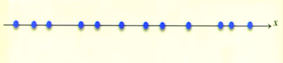
\includegraphics{lecture61}
\item In 1-D the closest pair of points must be adjacent in the x-ordering.\\
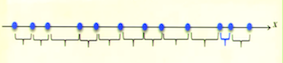
\includegraphics{lecture62}
	\begin{itemize}
	\item Thus we need to calculate only n-1 pairwise distances.
	
	\item Runtime (If the points are already sorted in x-order) = $O(n^2)$
	\item Runtime (If we have to sort the points first) = $O(n \cdot \log{}n)$
	\end{itemize}
\end{itemize}


\section{The 2-Dimensional Case}
\renewcommand{\labelitemii}{$\circ$}
\renewcommand{\labelitemiii}{$\cdot$}
\renewcommand{\labelitemiii}{$\rightarrow$}
\renewcommand{\labelitemiv}{$\star$}
\begin{itemize}
\item Let mimic this idea in 2-D on the point set $P = \{p_1, p_2, \cdot \cdot \cdot p_n\}$
	\begin{itemize}
	\item Order the points by their x-coordinate; we call this x-ordering.
	\item Order the points by their y-coordinate; we call this y-ordering.
	\item Find the \textit{pair of points closest} in their x-coordinate.
	\item Find the \textit{pair of points closest} in their y-coordinate.
	\end{itemize}

\item Does this algorithm work?
\begin{center}
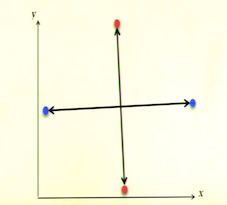
\includegraphics{lecture63}
\end{center}
	\begin{itemize}
	\item NO!
	\item This algorithm does not work: points that are close in their x-coordinate (or y-coordinate) may be very far apart.
	\item In fact, the closest point $P_i$ and $P_j$ can be seperated by many places in both the x-ordering and the y-ordering.
	\end{itemize}
\begin{center}
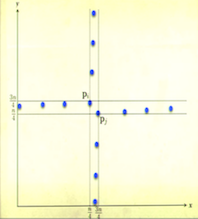
\includegraphics{lecture64}
\end{center}
\end{itemize}
	
\section{A Second Attempt}
\renewcommand{\labelitemii}{$\circ$}
\renewcommand{\labelitemiii}{$\cdot$}
\renewcommand{\labelitemiii}{$\rightarrow$}
\renewcommand{\labelitemiv}{$\star$}
\begin{itemize}
\item Instead let's try a \textbf{divide and conquer} approach.
\item Partition the points into \textit{two groups} of cardinality {\large $\frac{n}{2}$}.
	\begin{itemize}
	\item One way to do this is via the x-ordering using a \textbf{dividing line} D.
	\item We select D to pass through the point with the \underline{median} x-coordinate.
		\begin{itemize}
		\item We have a linear time algorithm to find the median.
		\end{itemize}
	\end{itemize}
\begin{center}
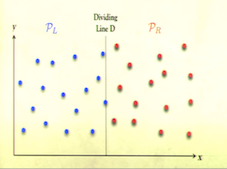
\includegraphics{lecture65}
\end{center}
\item Three Possibilities: 
	\begin{itemize}
	\item We can now recursively search for the closest pairs in $P_L$ and $P_R$.
	\end{itemize}
\begin{center}
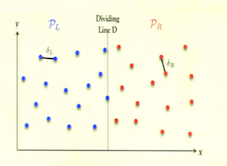
\includegraphics{lecture66}
\end{center}
\item But there is a \underline{third} possibility:
	\begin{itemize}
	\item The closest pair could have one point in $P_L$ and the other in $P_R$.
	\item So after calculating $\delta_L$ and $\delta_R$, we must check there is no better solution between a point in $P_L$ and a point in $P_R$.
	\end{itemize}
\end{itemize}

\section{The Recursive Algorithm}
\renewcommand{\labelitemii}{$\circ$}
\renewcommand{\labelitemiii}{$\cdot$}
\renewcommand{\labelitemiii}{$\rightarrow$}
\renewcommand{\labelitemiv}{$\star$}	
\begin{itemize}
	\item We can now recursively search for the closest pair in $P_L$ and $P_R$.
	\begin{enumerate}
	\item Find the point $q$ with the \textbf{median} x-coordinate.
	\item Partition $P$ into $P_L$ and $P_R$ using point $q$.
	\item Recursively find the \textit{closest pairs} of points in $P_L$ and $P_R$.
	\item Find the \textit{closest pair} with one point in $P_L$ and one point in $P_R$.
	\item Amongst the three pairs found, output the \textbf{closest} pair.
	\end{enumerate}
\item How long does this algorithm take?
	\begin{itemize}
	\item The recursive formula for the running time is:
	$$T(n) = 2 \cdot T(\frac{n}{2}) + O(n^2)$$
		\begin{itemize}
		\item Thus we have a = 2, b = 2, and d = 2.
		\item This is Case 1 of the Master Theorem.
		\item Runtime = $O(n^d) = O(n^2)$
		\end{itemize}
	\item The bottleneck operation is Step 4.
		\begin{itemize}
		\item So it takes far too long to measure the distance between every point in $P_L$ and every point in $P_R$.
		\item But, by solving the subproblems of $P_L$ and $P_R$, we know the \textbf{minimum pairwise distance} is at most: 
		$$ \delta = min\{\delta_L. \delta_R\}$$
		\item The trick is to use the value of $\delta$ (which we have calculated by recursion) to \underline{reduce} the number of distances we measure between $P_L$ and $P_R$.
		\item The key observation is that to find a better solution than $\delta$ the two points in $P_L$ and $P_R$ must be very close to the \textbf{dividing line} D...
		\begin{center}
		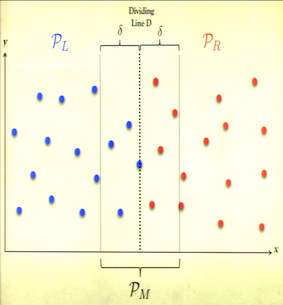
\includegraphics{lecture67}
		\end{center}
		\end{itemize}
	\end{itemize}
\item \textbf{Lemma.} Take $p_i \in P_L$ and $p_j \in P_R$. If $d(p_i, p_j) \leq \delta$ then $\{p_i, p_j\} \subseteq P_M$\\
\\
\textbf{Proof.} 
	\begin{itemize}
	\item Without lost of generality, assume $p_i \not\in P_M$
	\item Then $d(p_i,p_j) > \delta$
	\end{itemize}
\item So if the closest-pair is not in one of the two sub-problems then it is within $P_M$.
\begin{center}
	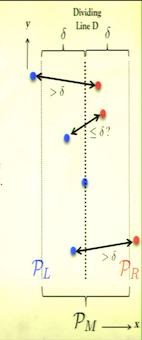
\includegraphics{lecture68}
\end{center}
\end{itemize}
	
\section{A modified Recursive Algorithm}
\renewcommand{\labelitemii}{$\circ$}
\renewcommand{\labelitemiii}{$\cdot$}
\renewcommand{\labelitemiii}{$\rightarrow$}
\renewcommand{\labelitemiv}{$\star$}	
\begin{itemize}
\item This induces the following \underline{fine-tuned} divide and conquer algorithm.
	\begin{enumerate}
	\item Find the point $q$ with the \textbf{median} x-coordinate.
	\item Partition $P$ into $P_L$ and $P_R$ using point $q$.
	\item Recursively find the \textit{closest pairs} of points in $P_L$ and $P_R$.
	\item Find the \textit{closest pair} of points in $P_M$. (Modified step!)
	\item Amongst the three pairs found, output the \textbf{closest} pair.
	\end{enumerate}
\item Problem?
	\begin{itemize}
	\item But $P_M$ may contain \textbf{all} (or most) of the points!
		\begin{itemize}
		\item It may still take time $\Omega(n^2)$ to measure the distances between the points in $P_L \cap P_M$ and the points in $P_R \cap P_M$
		\end{itemize} 
	\end{itemize}
\item But the points in $P_M$ cover a narrow band of the x-axis. As we have a \textbf{target} distance of $\delta$, this helps a lot...
	\begin{itemize}
	\item Consider the area of the plane within distance of $\delta$ of the line D.
	\item Divide this area up into small squares of width {\large $\frac{\delta}{2}$} as shown.\\
	\\
	\textbf{Claim.} No two points of $P$ lie in the same square.
	\\
	\item To prove this claim we will use the following observation.\\
	\\
	\textbf{Observation.} Each square lies entirely on one side of D.
	\\
\begin{center}
	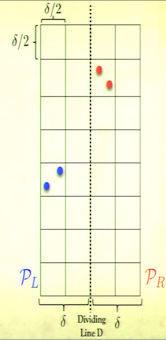
\includegraphics{lecture69}
\end{center}	
\textbf{Claim.} No two points of $P$ lie in the same square.\\
\textbf{Proof.}
		 \begin{itemize}
		\item \textit{wlog} Take two points in a square in $P_L$.
		\begin{center}
		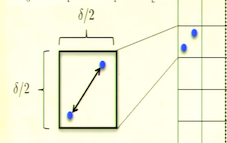
\includegraphics{lecture610}
		\end{center}
		\item Their pairwise distance is: {\large $\leq \sqrt{(\frac{\delta}{2})^2 + \frac{\delta}{2})^2} = \frac{\delta}{\sqrt{2}} < \delta$}
		\item This contradicts the fact that the smallest pairwise distance in $P_1$ is at least $\delta$.
		\end{itemize}
	\end{itemize}
	
\item \textbf{Theorem.} Take $p_i \in P_L$ and $p_j \in P_R$. If $d(p_i, p_j) \leq \delta$ then $p_i$ and $p_j$ have at most 10 points between them in the y-order of $P_M$.\\
\textbf{Proof.}
	\begin{itemize}
	\item \textit{wlog} $p_i$ is below $p_j$ in the y-order.
	\item Then $p_j$ is in the same row of squares as $p_i$ or in the next two higher rows.
	\item If not, $d(p_i, p_j) > \delta$, a contradiction.
	\begin{center}
	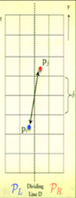
\includegraphics{lecture611}
	\end{center}
	\item But, by the claim, there is at most one point in each square.
		\begin{itemize}
		\item There are at most 10 points between $p_i$ and $p_j$ in the y-order of $P_M$.
		\end{itemize} 
	\end{itemize} 
\end{itemize}	
	
\section{Back to the 1-D Case}
\renewcommand{\labelitemii}{$\circ$}
\renewcommand{\labelitemiii}{$\cdot$}
\renewcommand{\labelitemiii}{$\rightarrow$}
\renewcommand{\labelitemiv}{$\star$}	
\begin{itemize}
\item This means the basic idea for the 1-D algorithm will work here!
\item To find the \textbf{closest pair} in $P_M$, we first sort the points by y-coordinate.\\
\\
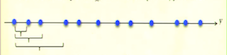
\includegraphics{lecture612}
\item Then, rather than finding the distances between points that are 1-apart in the y-order, we find the distances for all pairs up to 11 places apart.
\item Thus we calculate less than 11n pairwise distances. After doing so:
	\begin{itemize}
	\item Either we find a pair of points at distance less than $\delta$.
	\item Or we conclude that \textbf{no} such pair of points exists.
	\end{itemize} 
\item So give $\delta = min\{\delta_L, \delta_R\}$, we can check if there is a pair of points between $P_L$ and $P_R$ that are closer than $\delta$ in time $O(n)$.
\end{itemize}
\section{An Enhanced Modified Recursive Algorithm}
\renewcommand{\labelitemii}{$\circ$}
\renewcommand{\labelitemiii}{$\cdot$}
\renewcommand{\labelitemiii}{$\rightarrow$}
\renewcommand{\labelitemiv}{$\star$}	
\begin{itemize}
\item Finally, this will give us very fast divide and conquer algorithm.
	\begin{enumerate}
	\item Find the point $q$ with the \textbf{median} x-coordinate.
	\item Partition $P$ into $P_L$ and $P_R$ using point $q$.
	\item Recursively find the \textit{closest pairs} of points in $P_L$ and $P_R$.
	\item Find the \textit{closest pair} of points in $P_M$ using the \textbf{enhanced} 1-D algorithm. (Modified step!)
	\item Amongst the three pairs found, output the \textbf{closest} pair.
	\end{enumerate}
\item The recursive formula for the running time is:
	 {\large $$T(n) = 2 \cdot T(\frac{n}{2}) + O(n) $$}
	 \begin{itemize}
	\item Find median wrt x-coordinates.
	\item Partition into $P_L$ and $P_R$.
	\item Find $P_M$.
	\item Apply 1-D algorithm on $P_M$.
	\end{itemize} 
\item Thus we have a = 2, b = 2, and d = 1.
\item This is Case 2 of the Master Theorem.
\item Runtime = $O(n^d \cdot \log{}n) = O(n \cdot \log{}n)$
\item Validity of the algorithm:
	\begin{itemize}
	\item As usual, the correctness of the algorithm follows by \textit{strong induction}.
	\item For the \textbf{bases cases}, we can find the closest pair in constance time by exhaustive search when there are a constant number of points left.
	\item That the \textbf{inductive step} is correct follows by our discussion in the lecture.
		\begin{itemize}
		\item \textbf{Theorem.} The recursive algorithm finds the minimum distance pair of points.
		\end{itemize} 
	\end{itemize} 
\end{itemize}
	
	
\section{Computational Geometry}
\renewcommand{\labelitemii}{$\circ$}
\renewcommand{\labelitemiii}{$\cdot$}
\renewcommand{\labelitemiii}{$\rightarrow$}
\renewcommand{\labelitemiv}{$\star$}
\begin{itemize}
\item The closest pair of points problem was a foundation question in the field of \textbf{computational geometry}.
\item Computational has numerous applications:
	\begin{itemize}
	\item Computer Graphics.
	\item Computer Vision.
	\item Geometric Information Systems.
	\item ...
	\end{itemize} 
\end{itemize} 	
	
	
	
	
	
	
	
	
	
\end{document}